\section{Introduction}
The goal of this project work was to implement a peripheral driver for the STM32F407 microcontroller \cite{RefManual}. The implemented driver enables the use of the analog-to-digital converter (ADC). The microcontroller which contains the analog-to-digital converter is located on a development board (STM32 F4 Discovery kit) shown in figure \ref{fig:Board}. This development board contains components that can be interfaced with the microcontroller.\\

\begin{figure}[htbp]
  \centering
     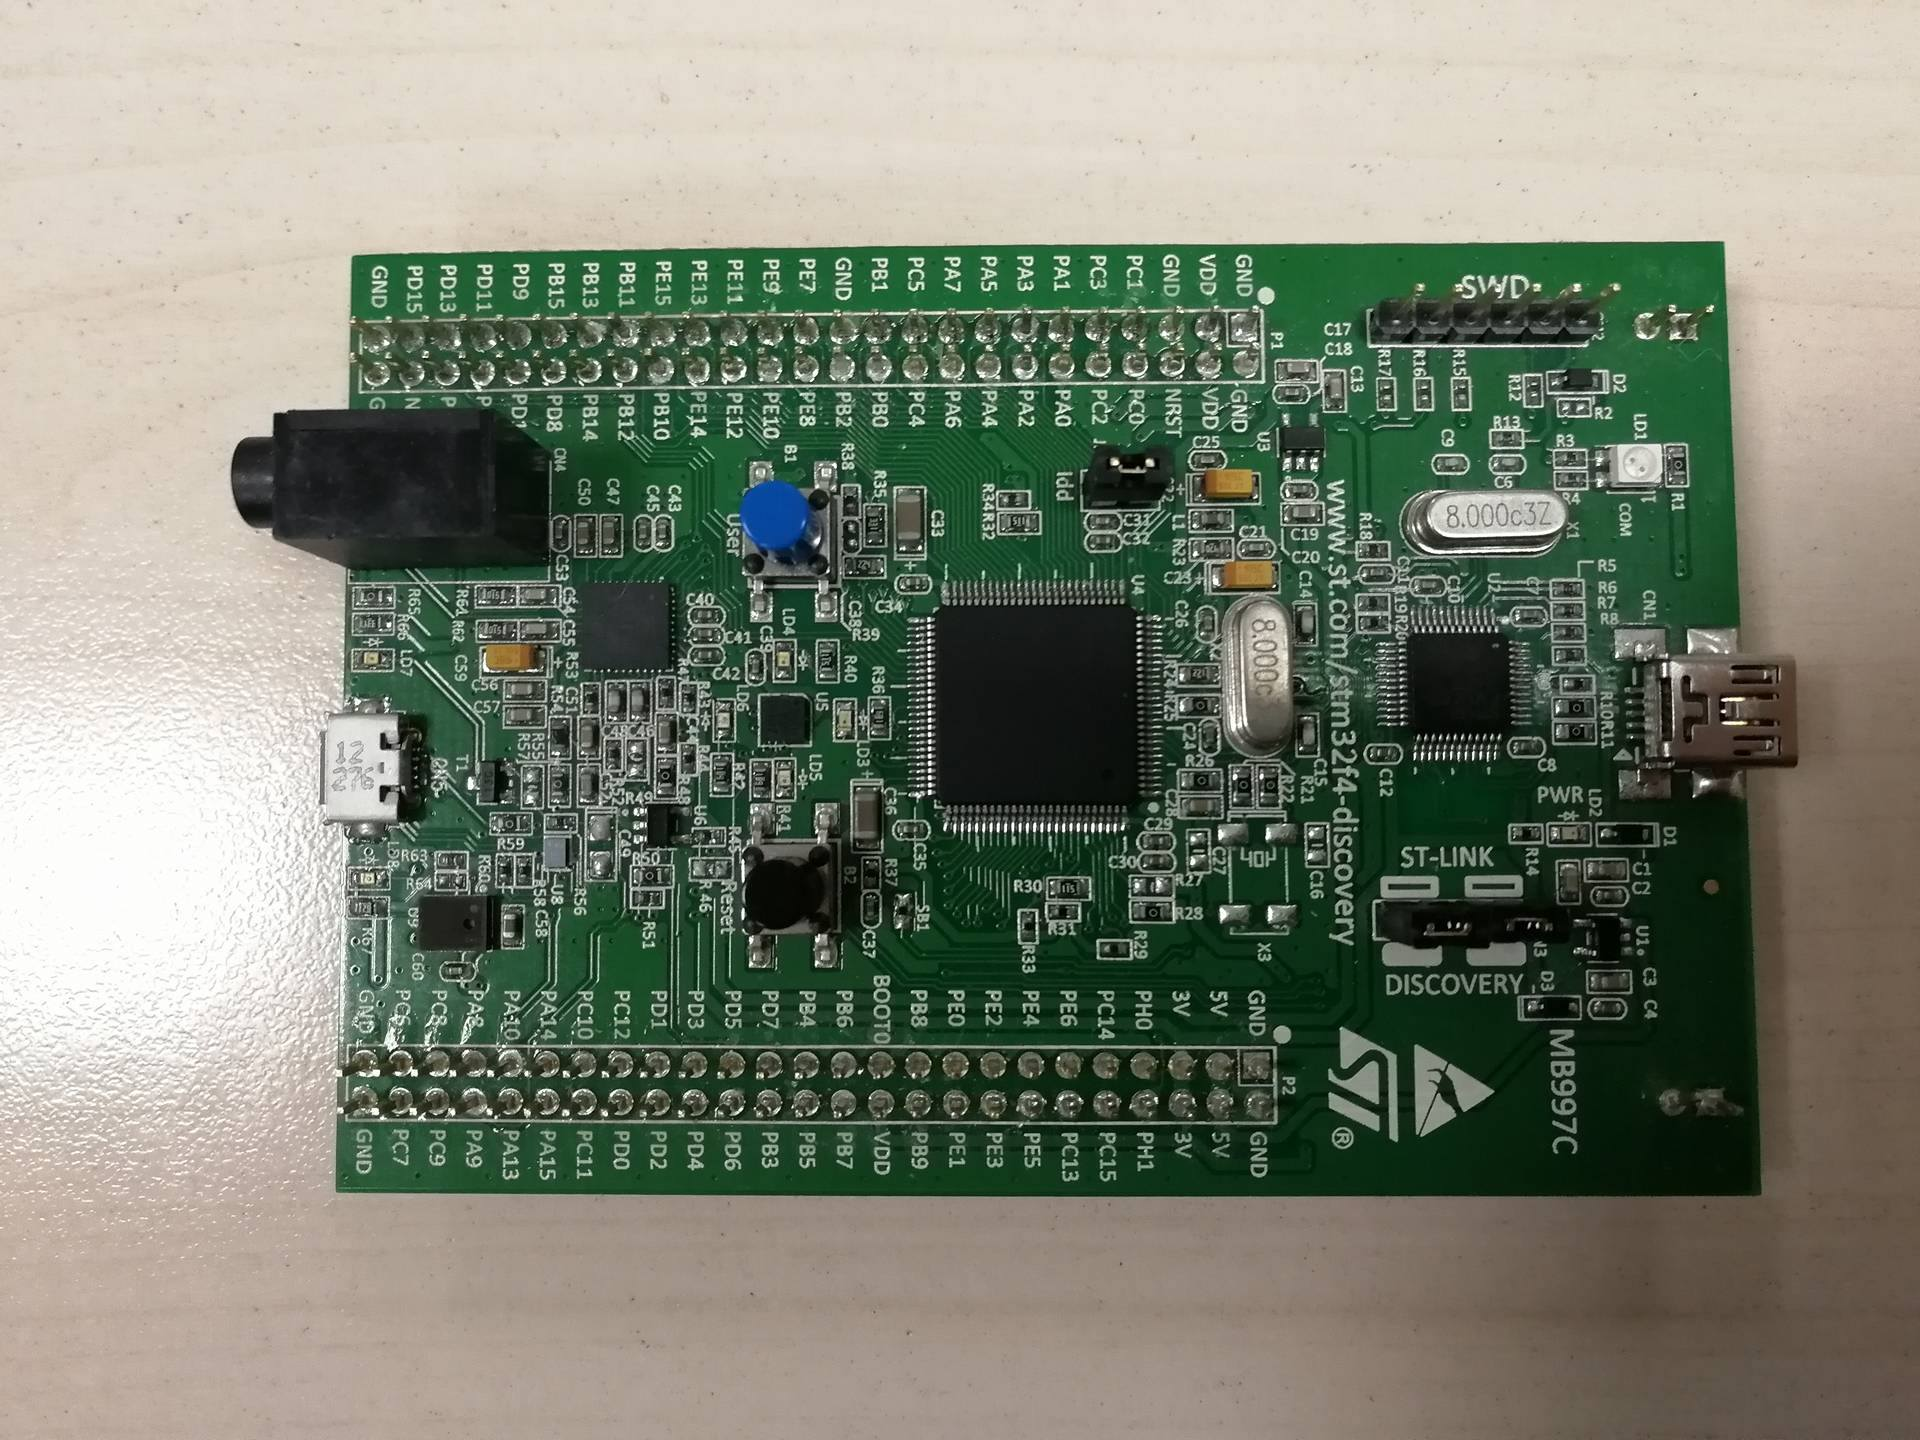
\includegraphics[width=0.7\textwidth]{./figures/board.jpg}
  \caption{Discovery Board}
  \label{fig:Board}
\end{figure}

\begin{figure}[htbp]
  \centering
     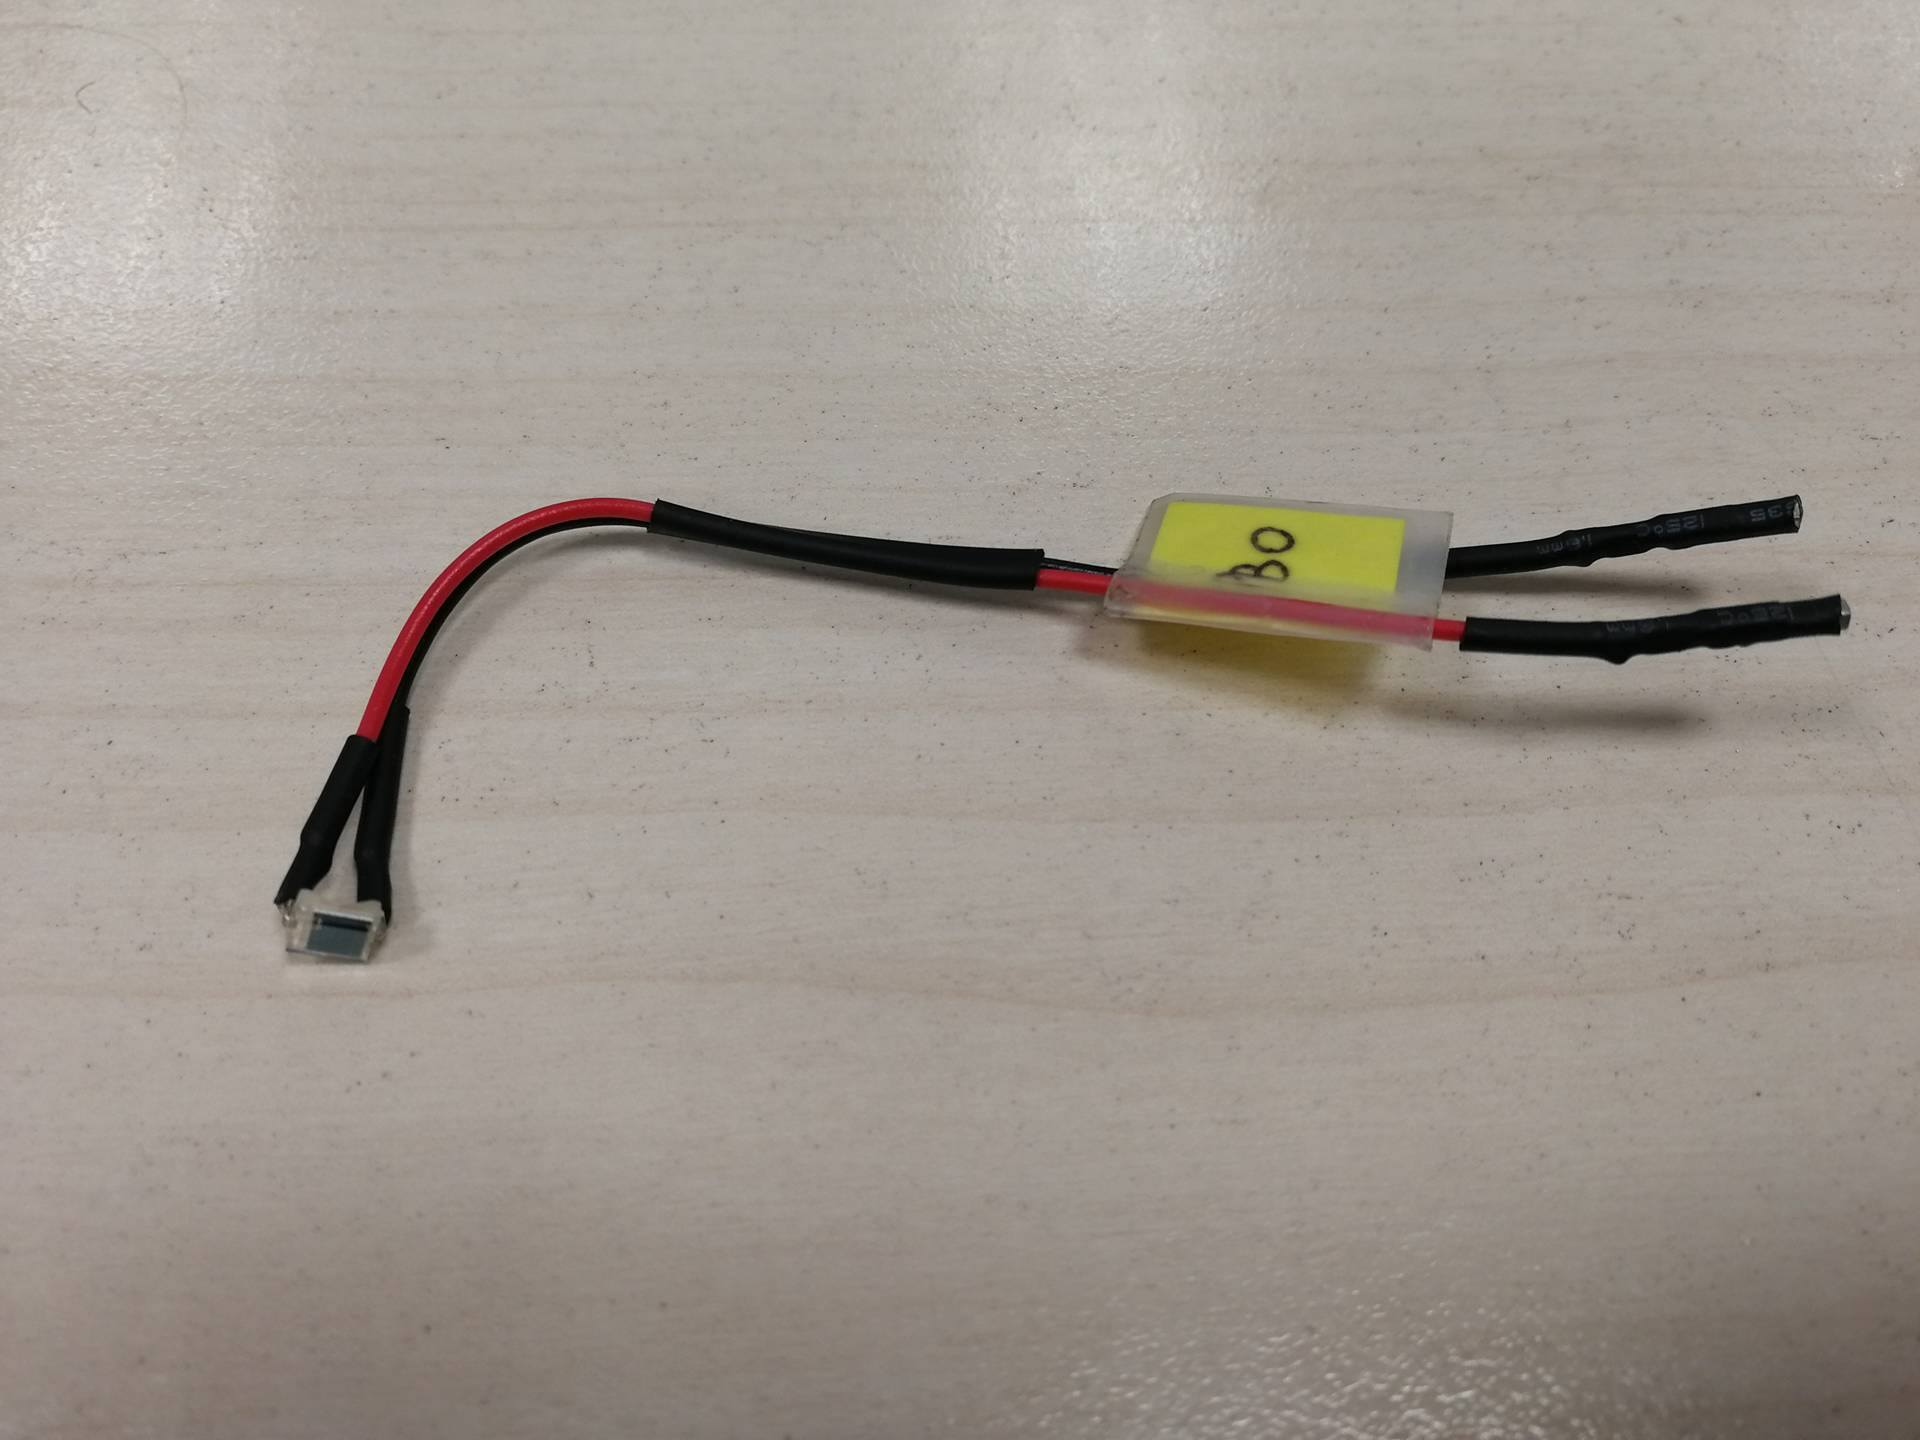
\includegraphics[width=0.5\textwidth]{./figures/photodiode.jpg}
  \caption{Photodiode}
  \label{fig:photodiode}
\end{figure}

\par
In this work the push button and user configurable LEDs of the development board were utilized as well as a external photodiode shown in figure \ref{fig:photodiode}. This photodiode was connected to the development boards external headers that enable connecting devices to the microcontroller. The photodiode and the components mentioned above were used to make a simple game that measures the user's reaction time.

\pagebreak


\section{Design and implementation}
\subsection{Game logic}
The idea of the implemented game was to test the reaction time of a player. This game can be played by a defined number of players. The reaction time of a player is evaluated by indicating a start signal and after this signal the player has to cover the photodiode as fast as possible to indicate a stop signal. The game logic is illustrated in figure \ref{fig:GameLogicDiagram}. 

\begin{figure}[htbp]
  \centering
     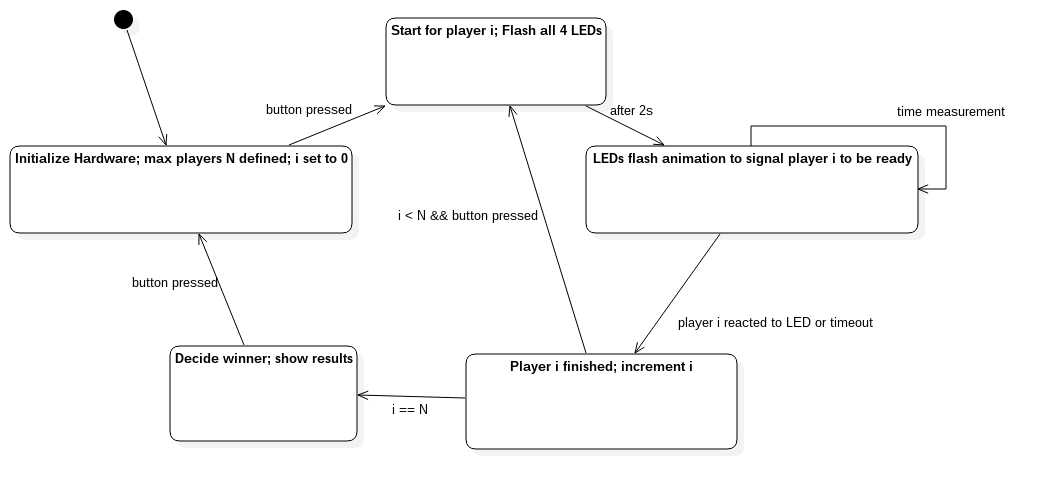
\includegraphics[width=1\textwidth]{./figures/FSM_Diagram.png}
  \caption{Game logic diagram}
  \label{fig:GameLogicDiagram}
\end{figure}

As illustrated in figure \ref{fig:GameLogicDiagram} the game can be started after the hardware initialization has been completed. The game is started when the board's user push button has been pressed. Information about the game status and corresponding instructions are printed on a serial monitor. These instructions are shown later on in this paper in chapter \ref{Results}.\\
\par
After the push button has been pressed as mentioned in previous paragraph it is the first player's turn and all of the user programmable LEDs start to flash rapidly for a short duration and then the LEDs turn off. This is an indication to the player to get ready and to be prepared to cover the photodiode soon. After this the LEDs start to light up in a clockwise orientation one by one. Once the fourth LED has lighten up, the player has to cover the photodiode as quickly as possible. Player reaction time is measured starting from the fourth LED lighting up and to the point when the photodiode has been covered.\\ 
\par
Then another player starts their turn by pressing the push button and has to interact with the system in the same manner as the player before. This cycle is repeated until all of the players have had their turn. The reaction times are finally displayed and the player who has had the lowest reaction time wins the game. A new game can be started by pressing the push button.

\subsection{Peripheral drivers}
For simplicity a design choice for this microcontroller project was to avoid the use of multiple threads. Every game logic procedure is executed in a sequential order and only interrupts allow to break this cycle and trigger events concurrently.\\
\par
In this project, interrupts are used by timers to toggle LEDs and for button detection. For the analog watchdog polling is utilized.
This approach allows to sense if the user tries to cheat by covering the photodiode before the fourth LED start to flash. As an alternative to this it would be also possible to realize the watchdog with interrupts and toggle the LEDs with sleep delays.\\
\par
The Miosix operating system \cite{Miosix} is included in the project workspace and is mainly used for a simplified accessing of the STM32F4 peripheral addresses by calling provided register names. Also the \emph{Timer} class for measuring time and the \emph{Random Number Generator} are exploited.

\subsubsection{ADC}
The use of the analog-to-digital converter builds the core of the project. A simple photodiode is connected to the board and the photodiode introduces an analog input voltage level depending on the ambient light intensity. The voltage has to be detected and read out as a digital signal in defined time intervals. Since the actual values are not important for this project, there is no data processing necessary. The values simply have to be compared to a watchdog threshold voltage and if they exceed this threshold, further action should be initiated. The analog watchdog provided by the microcontroller is used to execute this comparison.\\
\par
To enable the analog-to-digital converter peripheral and to connect the general purpose input/output (GPIO) pin to the ADC peripheral a set of registers is needed to be configured. The desired implementation is to connect the light sensor to the first GPIO of port B (PB0) and connect that GPIO to the ADC.\\
\par
First the GPIO port where the light sensor is connected needs to be enabled. Since the light sensor is connected to PB0 pin, the port B clock must be enabled. This is achieved by setting the GPIOBEN bit in the RCC AHB1 peripheral clock enable register. In order to connect the GPIO to the ADC it is needed to configure the GPIO port to analog mode of the four possible operation modes. This is done by writing the value 11 to the pin number (0) in the GPIO port mode register.\\
\par
The ADC peripheral is set up after connecting the GPIO port to ADC. From the user manual of the development board \cite{UsrManual} the used GPIO could be connected to first two ADC registers of the three available ADC registers of the microcontroller. This GPIO is connected to the input channel 8 of the ADC. It was decided to use the ADC1 of the microcontroller thus the corresponding clock was needed to be enabled from the RCC APB2 peripheral clock enable register.\\
\par
After setting up the GPIO register to be used in analog mode and connecting the register to the ADC the following functionality of the ADC was chosen:
\begin{itemize}
  \item Resolution: 12 bits
  \item Prescaler: PCLK2/8
  \item Sampling time of input channel (8): 84 cycles
  \item Data alignment: right data alignment
  \item Conversion mode: continuous conversion mode
\end{itemize}
All functionalities stated above could be set specifically for the ADC1 register except the prescaler value that is set in the common ADC register. The threshold value for the analog watchdog is calibrated everytime the ADC is initialized. This threshold value is defined by measuring light intensity values and then averaging a sum of light intensity values to set the threshold value. The use of the watchdog functionality can be set specifically to be used in one of the three ADCs.

\subsubsection{Push button}
The user configurable push button (blue push button in figure \ref{fig:Board}) is used for starting a game after board setup, switching player turn and starting a new game after a game has finished. The push button on the development board is connected to the PA0 GPIO according to the user manual \cite{UsrManual} of the development board. The push button uses interrupts to signal the mircocontroller that it has been pressed. The setup and use of the interrupt routine was done by using functions provided by the Miosix operating system.

\subsubsection{LEDs \& Timer}
Since the toggling of the LEDs is realized with interrupts, the LED management explicitly includes a hardware timer. The \emph{Led} class knows three different operating modes: At the beginning of a game round all four LEDs flash rapidly, after that the number of blinking LEDs increase from 1 to 3 and finally after a random time interval also the fourth LED becomes active. For all these three modes only one timer (TIM3) needs to be utilized because the blinking procedures happen sequentially.\\
\par
For every sequence the function \emph{startLedTimer()} is called with a different time interval which sets the prescaler of the timer. Also the new LED mode is passed with the function. With the given mode every time the timer generates an overflow interrupt, the corresponding IRQ handler knows in which way the LEDs should be toggled.

\subsubsection{Serial}
The serial connection is utilized to display game instructions and the winner of the game in a terminal window of a machine. Communication with other devices is done by using the USART interface. The development board can be connected to a machine with a USB to TTL serial cable since the board itself doesn't a provide a way that the USART interface can communciate with USB. While using miosix the USART connections are predefined. The connection is made with pins PB10 and PB11 with PB10 being the transmitting side and PB11 being the receiving side. Also a operating voltage and ground was provided for the TTL cable. The messages sent by the microcontroller can be viewed with a terminal window application e.g. \emph{screen} and using a correct transmission rate (19200) indicated in the miosix source code.

\subsubsection{Connections}
The connections made are described in table \ref{table:1} and also shown in figure \ref{fig:connections}. Table \ref{table:1} describes the functionality of the GPIO used.

\begin{table}
\caption{Connection table}
\label{table:1}
\begin{center}
\begin{tabular}{ |c|c| } 
 \hline
 Connector on development board & Function\\ 
 \hline
 PB0 & Positive terminal of photodiode connected to ADC \\
 PB10 & USART Transmit \\
 PB11 & USART Receive \\
 GND & Negative terminal of photodiode and USART ground \\
 \hline
\end{tabular}
\end{center}
\end{table}

\begin{figure}[htbp]
  \centering
     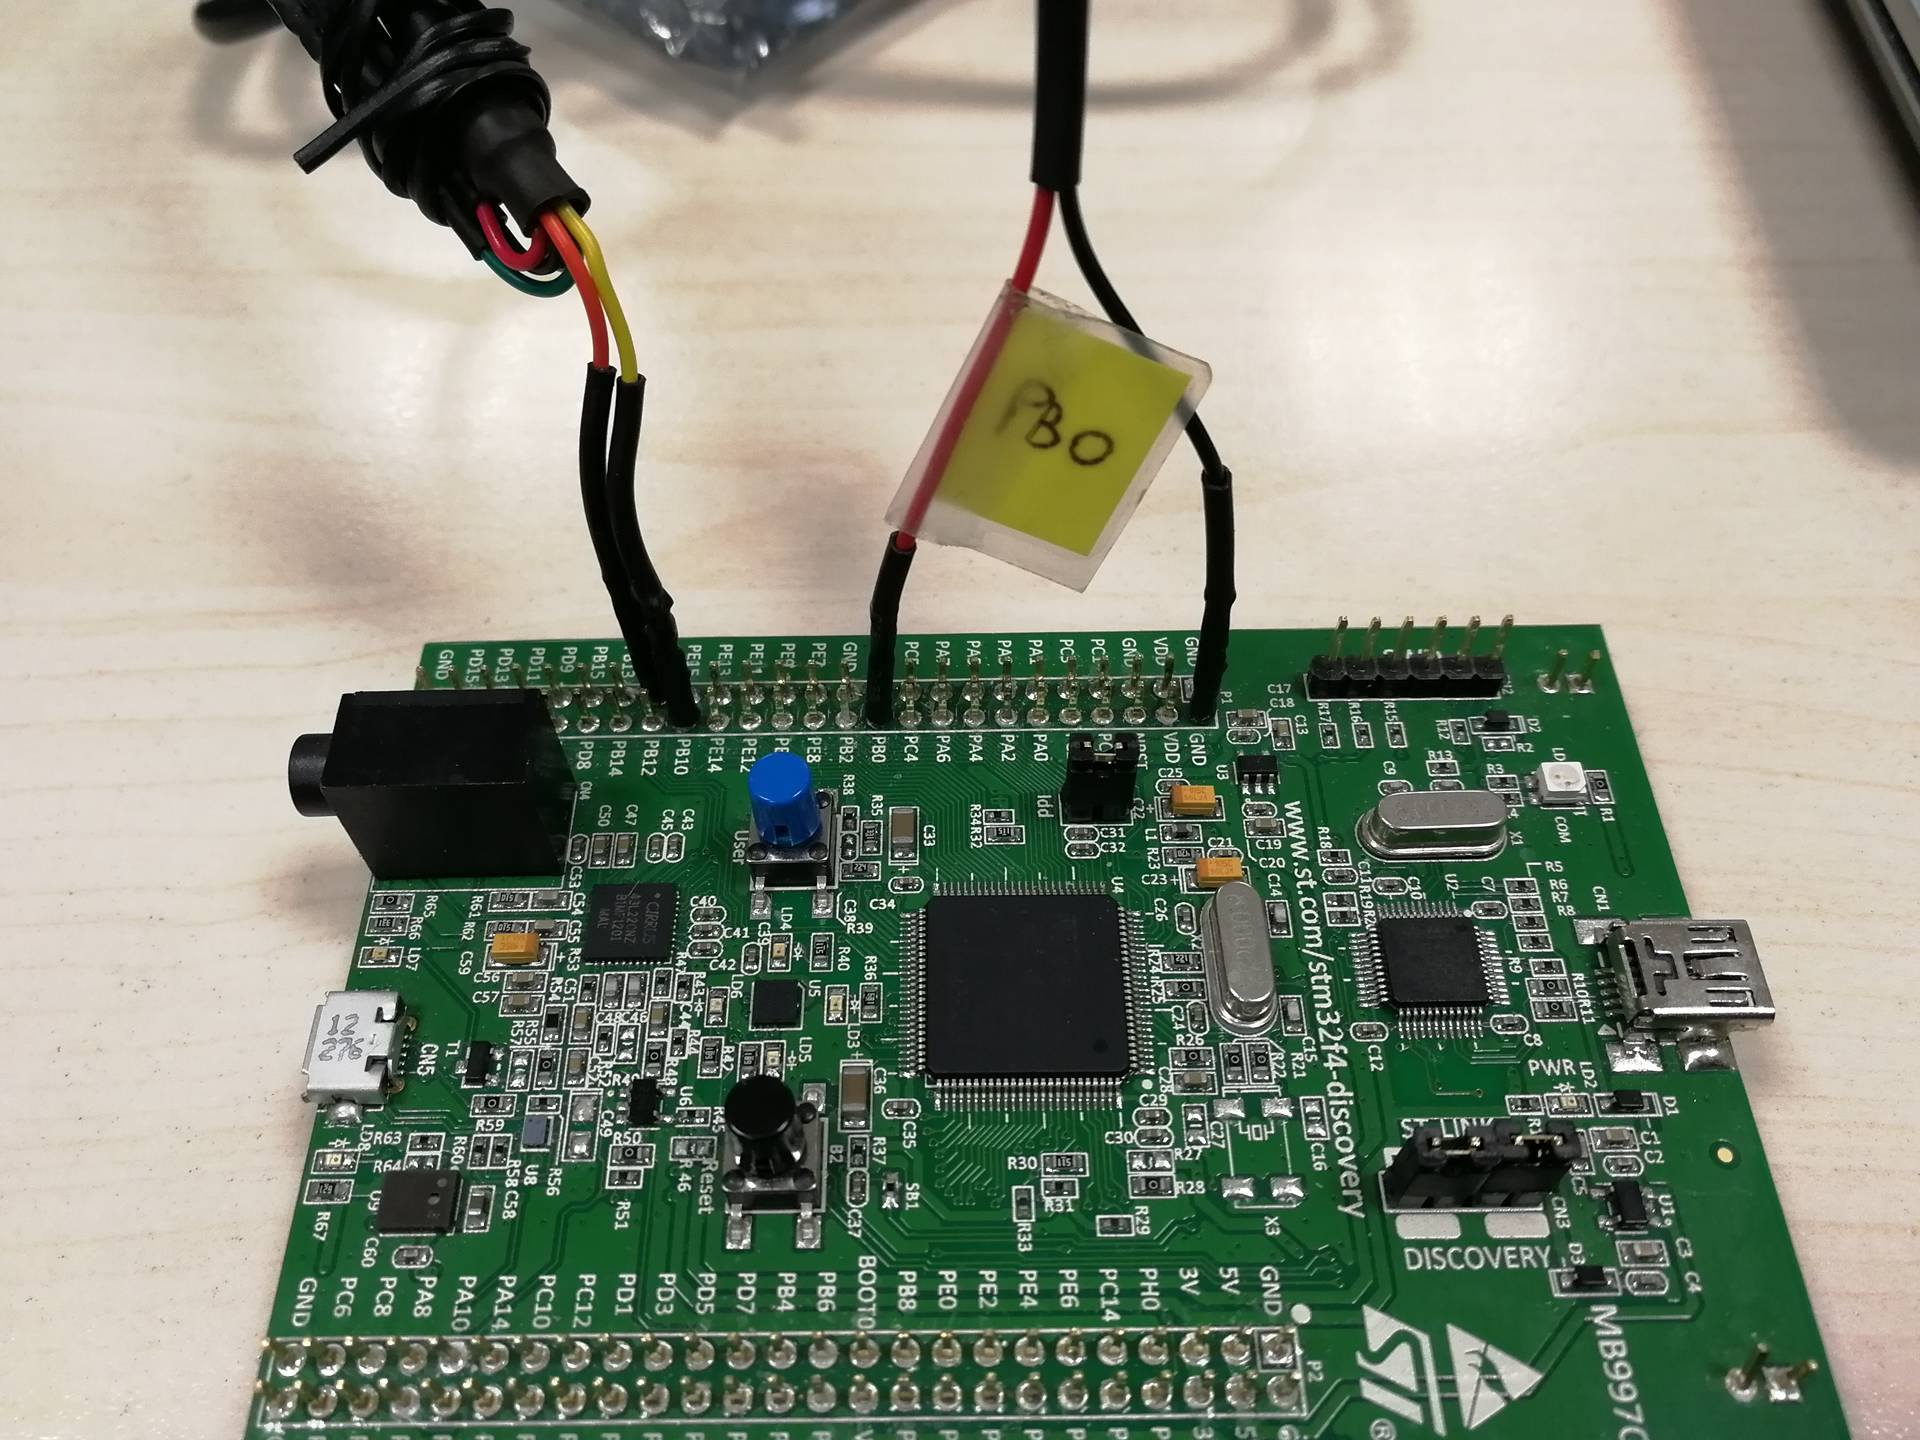
\includegraphics[width=1\textwidth]{./figures/connections.jpg}
  \caption{Connections}
  \label{fig:connections}
\end{figure}

\pagebreak

\section{Results} \label{Results}
The operation of the system was tested multiple times and also in different locations in order to test the analog watchdog threshold set correctness. After testing the system many times and in different locations the system was operating similarly every time and thus it was concluded that the system is working in the intended manner. The reaction time calculation correctness was tested comparing the results shown by the system and a manual stopwatch. This method isn't the most accurate one but the values were fairly similar so it was deemed to work correctly.\\
\par In the following figures \ref{fig:first_game_run} and \ref{fig:second_game_run} is a sample run of the game logic and starting a new game with pressing the push button after the first game has concluded.

\begin{figure}[htbp]
  \centering
     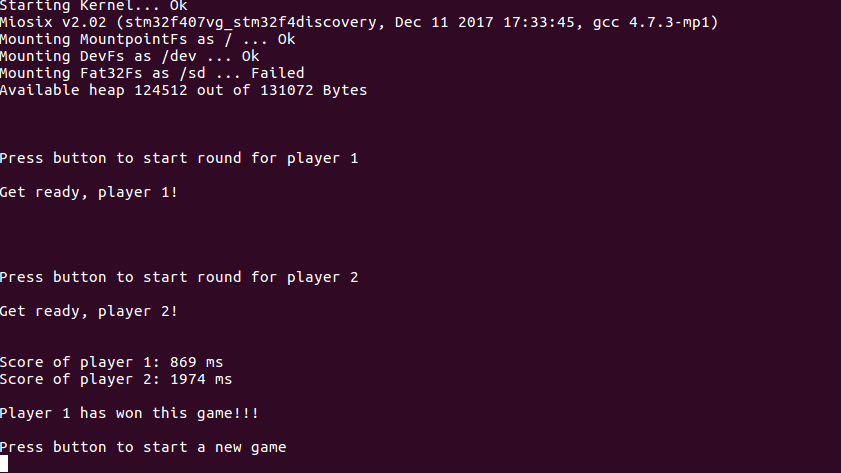
\includegraphics[width=1\textwidth]{./figures/Game_demo4.png}
  \caption{System setup and game logic}
  \label{fig:first_game_run}
\end{figure}

\begin{figure}[htbp]
  \centering
     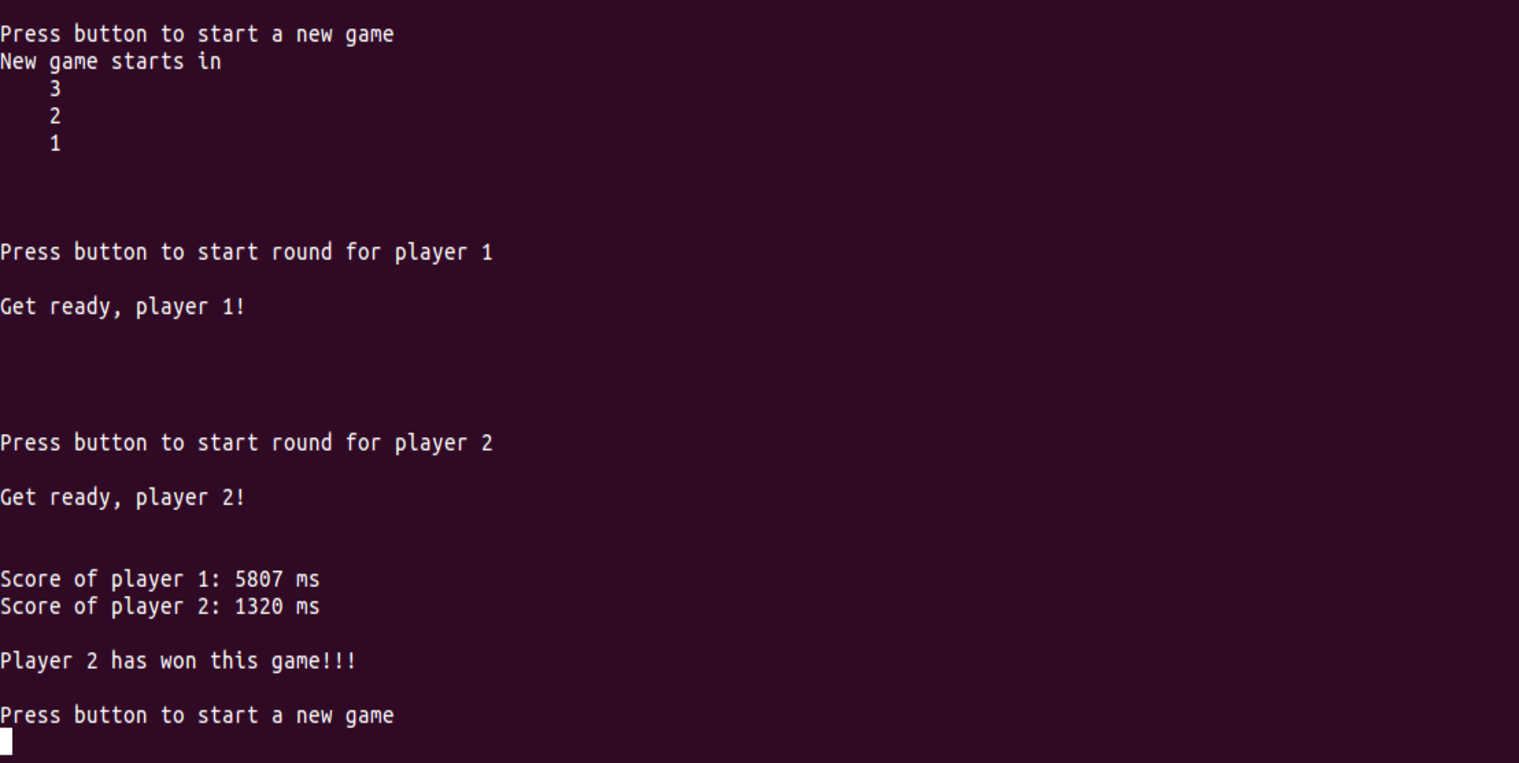
\includegraphics[width=1\textwidth]{./figures/Game_demo3.png}
  \caption{New game with pressing push button}
  \label{fig:second_game_run}
\end{figure}

\pagebreak


\section{Conclusions}
This project was about implementing an analog-to-digital converter driver for the STM32F407 microcontroller and interfacing it with a light sensor. Also the STM32 F4 Discovery kit development board was utilized to prdouce a user reaction time game with using the development boards user programmable LEDs and push button. The main emphasis of this project was to implement the ADC driver and the game was to utilize the converted values of the ADC. The system functionality was deemed to work as planned and thus satisfying the work's goals.